\label{sec:vbf-evtsel}

The event selection targets two different signal topologies:
\begin{itemize}
\item \fourcentral: both VBF jets and \bjets from the Higgs decay are 
  found in the central region of the detector ($|\eta|<2.8$)
\item \twocentral: at least one VBF jet is required to be
  in the forward region ($|\eta|>3.1$)
\end{itemize}

These two categories are designed to be exclusive and are fed by two separate trigger paths.  

\subsubsection{Trigger Definitions}
The \fourcentral category is fed by two triggers which were operational during different data taking periods.  The pre-ICHEP dataset (13 \ifb~in data periods A-D) utilized HLT\_2j45\_bmv2c2070\_split\_2j45, which requires four central Level-1 jet objects, referred to as regions of interest (ROI),  with \ET $>$ 15 \GeV~( L1\_4J15).  In the HLT two of these jets are required to have an HLT jet \ET of at least 45 \GeV~and be tagged with the 70\% working point of online $b$-tagging algorithm.  The integrated luminosity of this trigger is 9.38~\ifb. Post-ICHEP the  HLT\_2J35\_bmv2c60\_2J35 trigger is used, which also requires four central jets at Level-1  with Level-1 jet ROI \ET $>$ 15 \GeV~( L1\_4J15).  In the HLT two of these jets are required to have an HLT jet \ET of at least 35 \GeV~and be tagged with the 60\% working point of online $b$-tagging algorithm. The integrated luminosity of this trigger is 13.30~\ifb. The change was necessary in order not to exceed the allocated trigger bandwidth with the increasing luminosity conditions. The combined trigger efficiency (L1+HLT) for \fourcentral channel is 3.4\% for the signal sample. 

The \twocentral trigger is HLT\_j80\_bmv2c2070\_split\_j60\_bmv2c2085\_split\_j45\_320eta490 for the entire dataset.  At Level-1 it requires at least one central jet with a Level-1 ROI \ET of 40 \GeV~and $|\eta| < 2.5$.  Additionally it requires another central jet with ROI \ET $>$ 25 \GeV~and a third, forward jet with ROI \ET of at least 20 and   $3.1 < |\eta| < 4.9$.   At the HLT one central jet \btagged  with the 70\% online working point with at least 80 \GeV~is required, in addition to a second jet with at least 60 \GeV~tagged at the looser 85\% working point. Lastly, the forward jet is required to have \ET $>$ 45 \GeV~at the HLT. The combined trigger efficiency (L1+HLT) for \twocentral channel is 1.3\% for the signal sample. 



\subsubsection{Event Pre-Selection and Jet Assignment}
\label{sec:vbf-presel}
The analysis event pre-selection and jet assignment for each channel is as follows:

\paragraph{\fourcentral:} Events are required to pass  HLT\_2j45\_bmv2c2070\_split\_2j45 if they were recorded pre-ICHEP, HLT\_2J35\_bmv2c60\_2J35 if they were recorded post ICHEP.  Then we require at least two offline jets with \pT $>$ 55 \GeV~and ($|\eta| < 2.5$) which pass the offline \btagging at the medium working point.  Next, these jets are required to be matched to the HLT trigger \btagged trigger objects.  Two additional jets with \pT $>$ 55 \GeV~and  ($|\eta| < 2.8$) are also required.  If there is a jet with \pT $>$ 60 \GeV~and 3.2 $< |\eta| <$ 4.4 the event is vetoed in order to preserve exclusivity between the two analysis channels.  

All pairs of \btagged jets passing the medium working point are considered and the high \pT pair becomes our Higgs candidate.  All pairs of non-\btagged jets are also considered and the highest invariant mass pair form the VBF jets.   
The VBF jet assignment fails where there are only four jets above the \pT threshold, of which three are $b$-tagged.
% is not possible for events with only four jets above the \pT threshold, of which three are $b$-tagged. 
These events are rejected. 
%We are investigating the possibility of loosening this requirement to gain efficiency and consistency with the \twocentral channel (see below). 

Lastly, only events with a Higgs candidate transverse momentum, \pTbb, %of 
greater than 150 \GeV~are considered.  This requirement is needed to remove kinematic sculpting of the \Mbb distribution in the low \Mbb region.  Figure~\ref{fig:mbb_ptcuts} shows the \Mbb distribution for a variety of \pTbb cuts for the  pre-selected events outside of the Higgs mass window (the background sample) for the \fourcentral channel on the left.  It can be seen that a broad ``bump" is present in the distribution between 200 and 300~\GeV~when no \pTbb cuts are applied.  

\paragraph{\twocentral:} Events are required to pass HLT\_j80\_bmv2c2070\_split\_j60\_bmv2c2085\_split\_j45\_320eta490.   We require at least one offline jet with \pT $>$ 95 \GeV~which is \btagged at the medium working point.  We also require at least one additional jet with \pT $>$ 70 \GeV~which passes the loose offline \btagging working point.  These two jets must be matched to the HLT \btagged objects.  In addition to these jets, at least one forward jet with \pT $>$ 60 \GeV~and 3.2 $< |\eta| <$ 4.4 is required.  Lastly, the event must have at least one more jet with \pT $>$ 20 \GeV~ and $|\eta| <$ 4.4.  

Jet assignment proceeds as follows.  All pairs of \btagged jets passing the loose working point which contain at least one jet passing the medium working point are considered and the highest \pT pair becomes our Higgs candidate.  The VBF jet candidates are formed from all pairs of jets passing pre-selection which are not part of the Higgs candidate pair,  including at least one of the forward jets from the pre-selection.  There is no requirement that these jets fail  the \btagging requirements. The highest invariant mass pair are labeled the VBF jets. 

Lastly, only events with a Higgs candidate transverse momentum, \pTbb, %of 
greater than 160 \GeV~are considered.  This requirement is needed to remove kinematic sculpting of the \Mbb{} distribution in the low \Mbb{} region.  \Mbb{} is correlated with \pTbb{}, and the \pTbb{} distribution has a turn-on due to the jet \pT requirements. Figure~\ref{fig:mbb_ptcuts} shows the \Mbb distribution for a variety of \pTbb cuts for the background sample for the \twocentral channel on the right.  As the \pTbb{} cut is increased, the distribution assumes a regular falling spectrum.  The sculpting is worse for the \twocentral channel than the \fourcentral channel due to the higher threshold jet requirements. 


The details of the event selection are summarized in Table~\ref{tab:evtsel}. 
Jet \pT thresholds and $|\eta|$ requirements are chosen so that the efficiency of selecting a jet at trigger level that would pass the offline selection is at least 97\%. Cut flows for both selections are displayed in Tables~\ref{tab:cutflow_4cen} and~\ref{tab:cutflow_2cen}.


\paragraph{0-tag samples:} Both the \fourcentral and \twocentral channels have corresponding 0-tag samples in which the offline jets are required to be anti-\btagged at the 85\% working point. These samples are used to determine the sensitivity when determining the signal and control BDT regions.   A relatively tight anti-tag is required in order to minimize any leakage of the signal into the 0-tag sample.  In these samples supporting triggers are used, which have the same Level-1 and HLT jet requirements, but no \btagging requirements.  These triggers are heavily pre-scaled.  


\paragraph{Overlap with VBF$+\gamma$ Analysis:} The result of this analysis will be combined with the complementary VBF$+\gamma$ analysis which studies the same event topology with an additional photon radiated by the initial/final state quarks or the vector bosons. For the two analyses to remain orthogonal, the inclusive analysis vetos events selected by the VBF$+\gamma$ analysis in data. From simulation it is determined that only 0.11\% and 0.047\% of the inclusive VBF signal MC would pass selections of both analyses given that they pass \twocentral and \fourcentral respectively. The size of this overlap is so small, less than $0.5\%$ (a criterion for us to account a particular source of systematics in the final fit \ref{sec:vbf-uncertainties}), such that it is neglected.  


\begin{figure}[htbp]
  \centering
 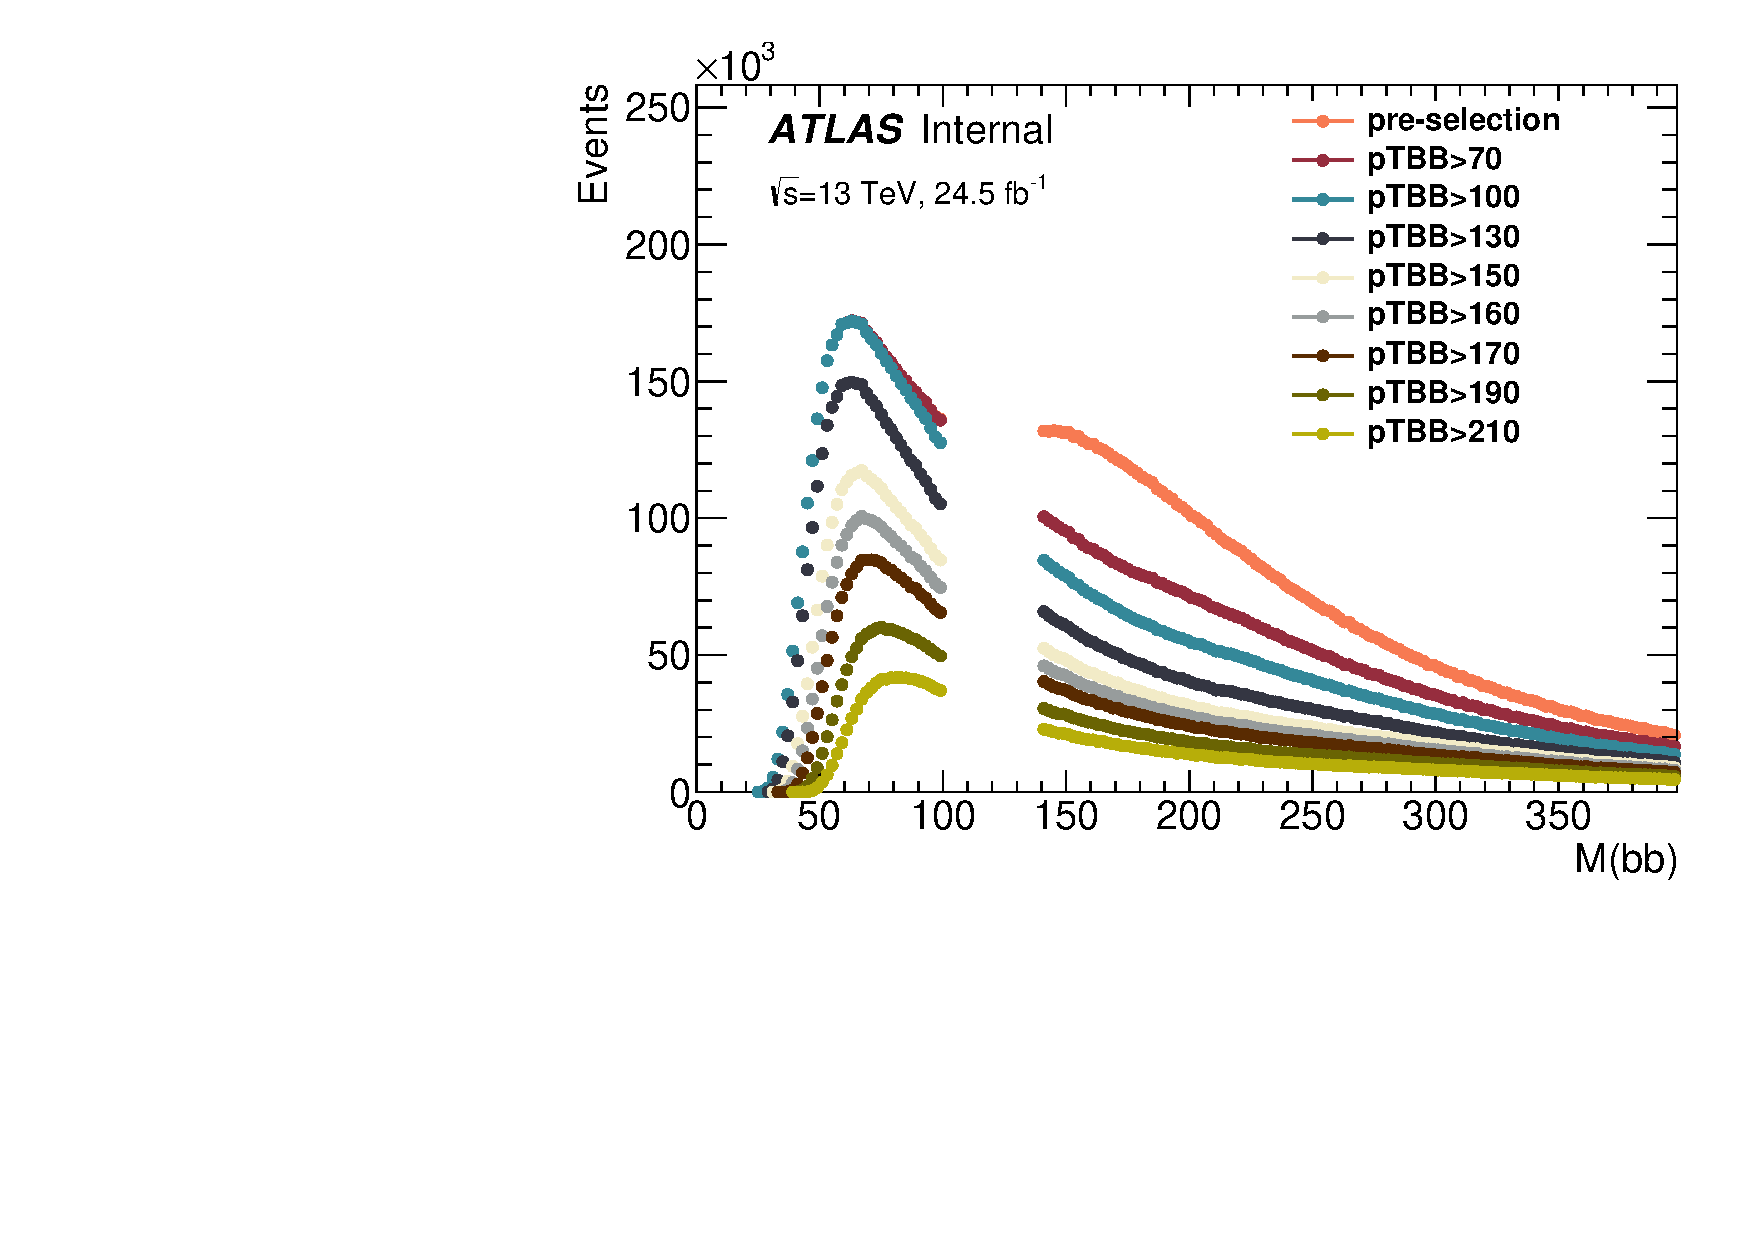
\includegraphics[width=0.45\textwidth]{figures/VBF/Presel-Mbb_4cen.pdf}
 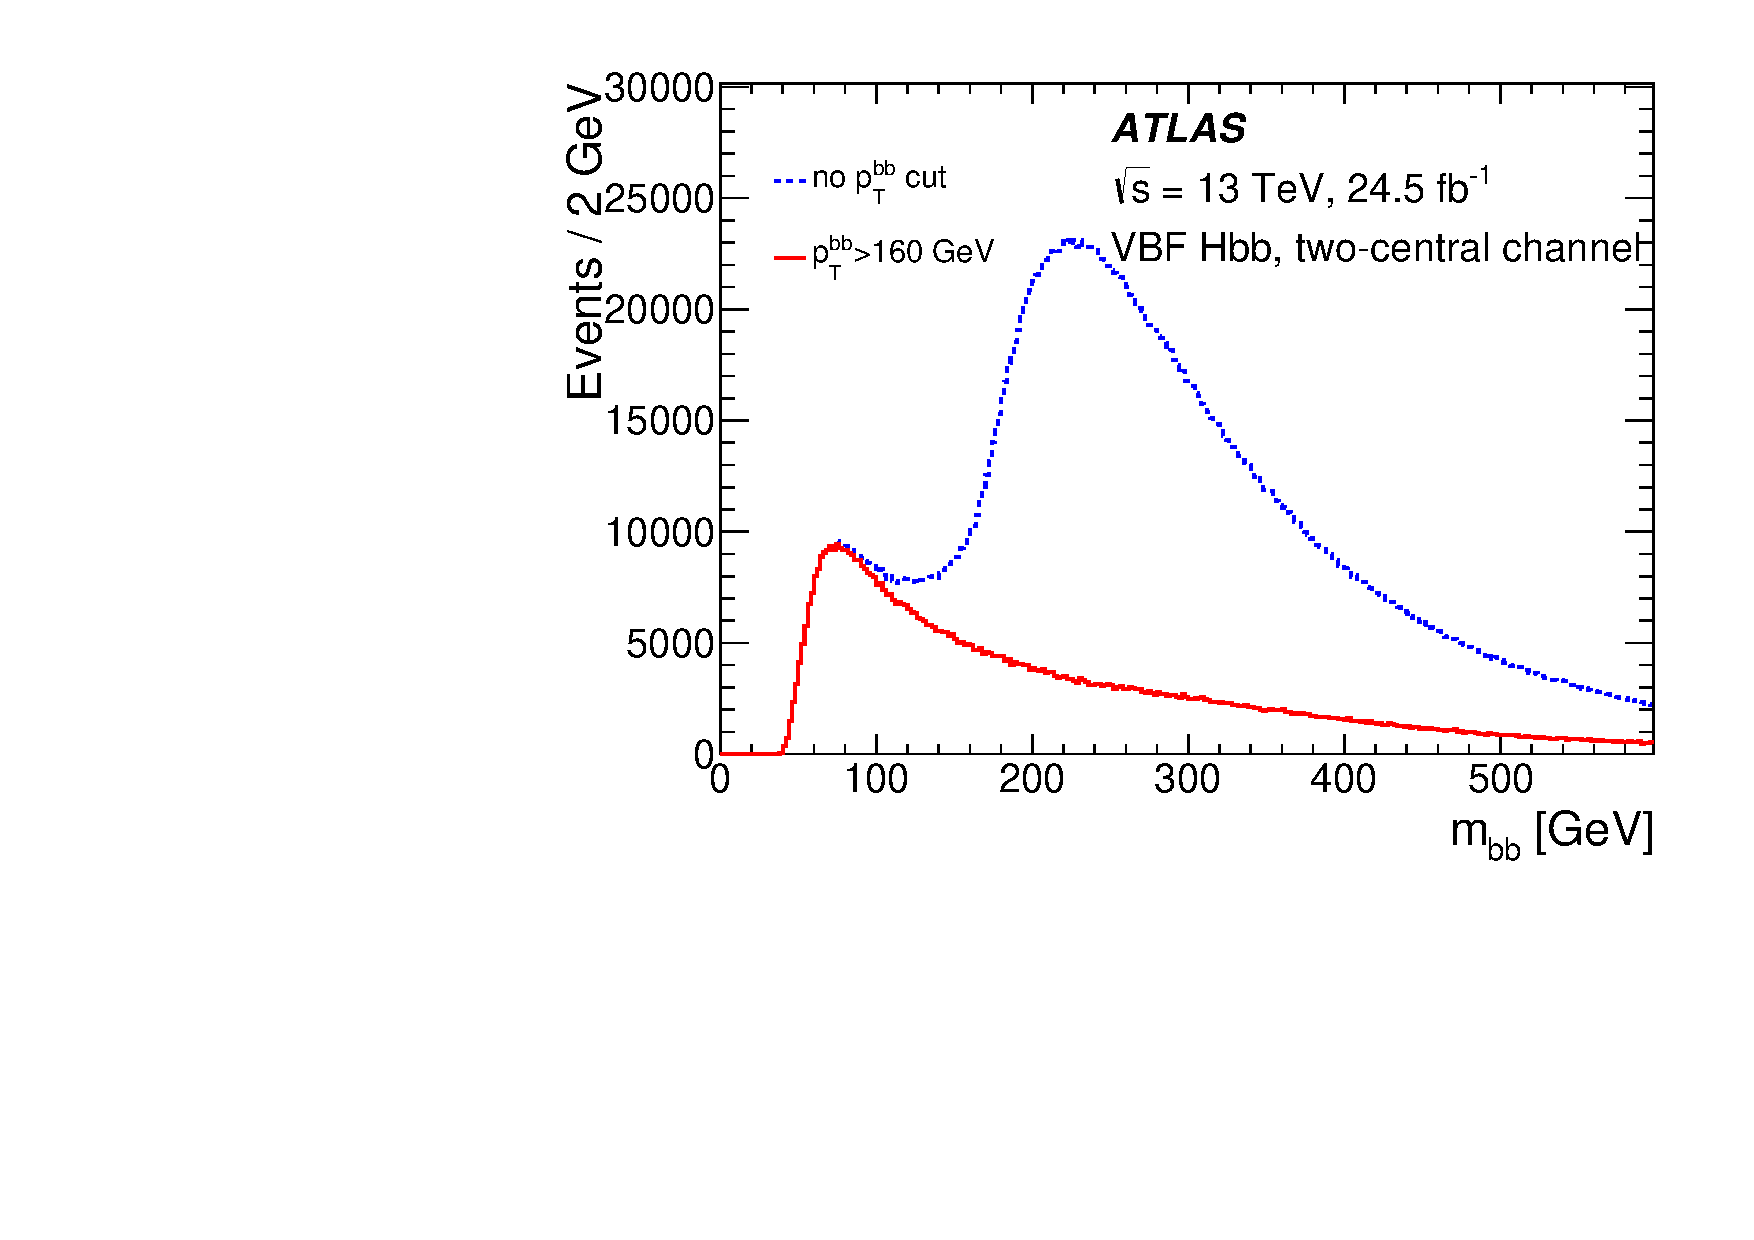
\includegraphics[width=0.45\textwidth]{figures/VBF/Presel-Mbb_2cen.pdf}
 \caption{Distributions of \Mbb for a variety of \pTbb cuts using data events.  \fourcentral events on the left, \twocentral on the right.  All event pre-selection criteria except the \pTbb cuts are applied.}
  \label{fig:mbb_ptcuts}
\end{figure}


%Then put into BDT & we have SR1, SR2 & CR.  Used to have 0 tag control sample but not used.

%The details of the event selection are summarized in Table~\ref{tab:evtsel}. 
With exception of the trigger requirements, the same requirements are placed on the data and MC samples.  In the MC15 samples the trigger decision is missing for the \twocentral channel, therefore an alternative emulation is used, described briefly in Section~\ref{sec:vbf-trig}.

\begin{table}[htbp]
  \begin{center}
    \resizebox{\textwidth}{!}{
      \begin{tabular}{ l  c c }
        \toprule
        & \fourcentral & \twocentral \\
        \midrule
        L1 trigger          & L1\_4J15                 & L1\_J40\_0ETA25\_2J25\_J20\_31ETA49                                \\
\\
        Primary HLT trigger  & HLT\_2j45\_bmv2c2070\_split\_2j45  & HLT\_j80\_bmv2c2070\_split\_j60\_bmv2c2085\_split\_j45\_320eta490  \\ 
                 & HLT\_2j35\_bmv2c2060\_split\_2j35  &   \\ 

      \\ 
        Support HLT trigger & HLT\_4j45                          & HLT\_j80\_0eta240\_j60\_j45\_320eta490                             \\ 
        \\
                                              &                                                     & $\geq4$ jets with $\pt>20$ \GeV{} and $|\eta|<4.4$ \\
                                              &                                                     & $\geq1$ jet with $\pt>60$ \GeV{} and $3.2<|\eta|<4.4$  \\ 
                                              &                                                     & $\geq2$ jets with $\pt>70$ \GeV{} and $|\eta|<2.5$ \\ 
        \multirow{-4}{*}{Jet selection}       & \multirow{-4}{*}{$\geq4$ jets with $\pt>55$ \GeV{} and $|\eta|<2.8$} & $\geq1$ jet with $\pt>95$ \GeV{} and $|\eta|<2.4$  \\ 
        \\
        
        \multirow{2}{*}{$b$-tagging}          & \multirow{2}{*}{$\geq2$ $b$-jets with $\pt>55$ \GeV{} and $|\eta|<2.5$} & $\geq2$ $b$-jets with $\pt>70$ \GeV{}                  \\ 
                                              &                                                        & $\geq1$ $b$-jets with $\pt>95$ \GeV{} and $|\eta|<2.4$ \\ 
        Forward jet veto                      &   No jet with $\pt>60$ \GeV{} and $3.2<|\eta|<4.4$    &  \\ 
        Higgs boson candidate                 &       $\pt(b\bar{b})>150$ \GeV{}                       &  $\pt(b\bar{b})>160$ \GeV{} \\  
        
        \bottomrule
      \end{tabular}
    }
  \end{center}
  \caption{Event selection for the two event categories. The \fourcentral has two primary trigger paths.  The first is used for the pre-ICHEP dataset, the second is used for the post-ICEP dataset. \bjets{} are tagged with the 70\% working point and are required to have $|\eta| < 2.5$}
  \label{tab:evtsel}
\end{table}



\begin{table}[]
\centering
  \caption{Cutflow for the \fourcentral events. The details of the cuts are found in the text. Jet assignment refers to the designation of jets as signal or VBF jets.  After the forward jet veto some \fourcentral events can fail the jet assignment. MC events are normalized to cross section times branching ratio.  The total number of data events is after the application of the derivation skimming whereas the MC events are the total number of events in the MC samples. *The data number of total events is the number of all events after the derivation skim.}
\label{tab:cutflow_4cen}
\begin{tabular}{|l|l|l|l|l|l|}
\hline
                       & \multicolumn{5}{c|}{Pre-ICHEP}                                 \\ \hline
                       & data 2tag  & VBF       & ggF        & Zbb(QCD)     & Zbb(EWK)  \\ \hline
Events                 & 122517049* & 20127.77 & 234762.76 & 3880727.12 & 29277.82 \\ \hline
Trigger                & 29623250   & 626.97    & 2192.08    & 98931.10    & 1444.48  \\ \hline
2 medium \btagged jets & 13910362   & 334.25    & 1207.25    & 45110.51    & 704.96    \\ \hline
$\ge$ 4 jets           & 9255271    & 215.23    & 892.07     & 35903.91    & 566.74    \\ \hline
Forward jet veto       & 9021208    & 205.80    & 869.90     & 34675.67    & 545.12    \\ \hline
Jet Assignment         & 8290467    & 197.22    & 820.17     & 33604.22    & 532.11    \\ \hline
$\pTbb>150\GeV$        & 3146579    & 121.82    & 532.44     & 21083.98    & 379.19    \\ \hline
Photon veto in data    & 3145966    & 121.82    & 532.44     & 21083.98    & 379.19    \\ \hline
                       & \multicolumn{5}{c|}{Post-ICHEP}                                \\ \hline
                       & data 2tag  & VBF       & ggF        & Zbb(QCD)     & Zbb(EWK)  \\ \hline
Events                 & 169139398* & 28565.54 & 332928.99 & 5505804.89 & 41551.38 \\ \hline
Trigger                & 43820814   & 1024.11   & 3602.91    & 166327.21   & 2271.46  \\ \hline
2 medium \btagged jets & 19370468   & 501.79    & 1868.41    & 64549.54    & 955.57    \\ \hline
$\ge$ 4 jets           & 10218887   & 273.80    & 1133.73    & 45143.89    & 712.79    \\ \hline
Forward jet veto       & 9963404    & 261.86    & 1105.68    & 43605.23    & 685.11    \\ \hline
Jet Assignment         & 9065632    & 250.22    & 1037.54    & 42162.97    & 667.93    \\ \hline
$\pTbb>150\GeV$        & 3755031    & 157.99    & 685.40     & 27202.75    & 486.46    \\ \hline
Photon veto in data    & 3754301    & 157.99    & 685.40     & 27202.75    & 486.46    \\ \hline
\end{tabular}
\end{table}



\begin{table}[]
\centering
  \caption{Cutflow for the \twocentral events. The details of the cuts are found in the text. Jet assignment refers to the designation of jets as signal or VBF jets.  In the \twocentral channel events cannot fail the jet assignment but the line is preserved here for consistency with the \fourcentral channel.  MC events are normalized to cross section times branching ratio. The total number of data events is after the application of the derivation skimming whereas the MC events are the total number of events in the MC samples. *The data number of total events is the number of all events after the derivation skim.}
  \label{tab:cutflow_2cen}
\begin{tabular}{|l|l|l|l|l|l|}
\hline
                            & data       & VBF       & ggF       & Zbb(QCD)    & Zbb(EWK)    \\ \hline
Events                      & 291656447* & 52628.646 & 613382.49 & 10143797.55 & 76540.41    \\ \hline
Trigger                     & 18425823   & 679.17    & 593.97    & 23942.09    & 555.71      \\ \hline
1 Medium \btagged jet       & 10321971   & 455.01    & 405.16    & 14816.09    & 369.59      \\ \hline
$\ge$ 2 loose \btagged jets & 3529025    & 269.69    & 244.54    & 7753.00     & 203.92      \\ \hline
Forward jet requirement     & 2814936    & 214.93    & 181.60    & 5328.06     & 162.68      \\ \hline
$\ge$ 4 jets                & 2527300    & 208.09    & 175.97    & 5307.56     & 161.70      \\ \hline
Jet Assignment              & 2527300    & 208.09    & 175.97    & 5307.56     & 161.70      \\ \hline
$\pTbb>160\GeV$             & 884095     & 147.27    & 126.50    & 3565.69     & 122.42      \\ \hline
Photon veto in data         & 883906     & 147.27    & 126.50    & 3565.69     & 122.42      \\ \hline
\end{tabular}
\end{table}

